\section{Igénybevételi függvények}

\newcommand*\circled[1]{\tikz[baseline=(char.base)]{
            \node[shape=circle,draw,inner sep=2pt] (char) {#1};}}

\newcommand{\strucstresscoorded}{%
	\draw[thick,->,gray] (0,0) -- ++(2,0) node[anchor=north west] {$x_\text{1}$};
	\draw[thick,->,gray] (0,0) -- ++(0,2) node[anchor=south east] {y};

	\draw[thick,->,gray] (\as + \bs + \cs,0) -- ++(0,2) node[anchor=south east] {$x_\text{2}$};
	\draw[thick,->,gray] (\as + \bs + \cs,0) -- ++(-2,0) node[anchor=north west] {y};

	\strucframe
	\strucforces
	\strucsharedforces
	\strucrestrainforces

	\draw ({(\as + \bs + \cs) / 2}, -.5) circle (.25) node {1};
	\draw (B)++(.5, -\ks / 2) circle (.25) node {2};
}

\begin{center}
        \begin{tikzpicture}
		\strucstresscoorded
        \end{tikzpicture}

	\vskip 20pt
	
	\begin{multicols}{2}
		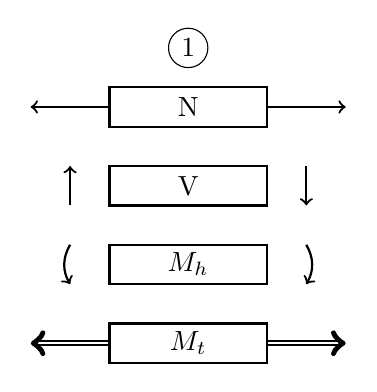
\begin{tikzpicture}
			\draw (1, 1) circle (.25) node {1};

			\draw[thick, <-] (0,.25)++(-1,0) -- (0,.25);
			\draw[thick, ->] (0,.25) -- ++(3,0);
			\fill[white] (0,0) rectangle ++(2,.5);
			\draw[thick] (0,0) rectangle ++(2,.5) node[midway] {N};

			\draw[thick, ->] (-.5,-1) -- ++(0,.5);
			\draw[thick, <-] (2.5,-1) -- ++(0,.5);
			\fill[white] (0,-1) rectangle ++(2,.5);
			\draw[thick] (0,-1) rectangle ++(2,.5) node[midway] {V};

			\draw[thick, <-] (-.5,-2) to [bend left] ++(0,.5);
			\draw[thick, <-] (2.5,-2) to [bend right] ++(0,.5);
			\fill[white] (0,-2) rectangle ++(2,.5);
			\draw[thick] (0,-2) rectangle ++(2,.5) node[midway] {$M_\text{h}$};
			
			\draw[thick, double, ->] (0,-2.75) -- ++(-1,0);
			\draw[thick, double, ->] (0,-2.75) -- ++(3,0);
			\fill[white] (0,-3) rectangle ++(2,.5);
			\draw[thick] (0,-3) rectangle ++(2,.5) node[midway] {$M_\text{t}$};
		\end{tikzpicture}

		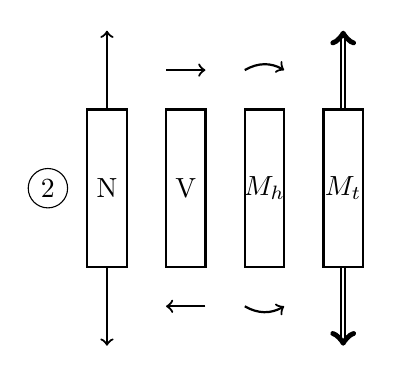
\begin{tikzpicture}[rotate=90]
			\draw (1, 1) circle (.25) node {2};

			\draw[thick, <-] (0,.25)++(-1,0) -- (0,.25);
			\draw[thick, ->] (0,.25) -- ++(3,0);
			\fill[white] (0,0) rectangle ++(2,.5);
			\draw[thick] (0,0) rectangle ++(2,.5) node[midway] {N};

			\draw[thick, ->] (-.5,-1) -- ++(0,.5);
			\draw[thick, <-] (2.5,-1) -- ++(0,.5);
			\fill[white] (0,-1) rectangle ++(2,.5);
			\draw[thick] (0,-1) rectangle ++(2,.5) node[midway] {V};

			\draw[thick, <-] (-.5,-2) to [bend left] ++(0,.5);
			\draw[thick, <-] (2.5,-2) to [bend right] ++(0,.5);
			\fill[white] (0,-2) rectangle ++(2,.5);
			\draw[thick] (0,-2) rectangle ++(2,.5) node[midway] {$M_\text{h}$};
			
			\draw[thick, double, ->] (0,-2.75) -- ++(-1,0);
			\draw[thick, double, ->] (0,-2.75) -- ++(3,0);
			\fill[white] (0,-3) rectangle ++(2,.5);
			\draw[thick] (0,-3) rectangle ++(2,.5) node[midway] {$M_\text{t}$};
		\end{tikzpicture}
	\end{multicols}
\end{center}

Körüljárással meglehet mind a két rúd igénybevételi függvényeit vizsgálni. Megfelelő \textcolor{gray}{koordináta-rendszerek} és előjelkonvenciók felvétele után az \circled{1}-es rudat balról, míg a \circled{2}-es rudat jobbról nézhetjük. (Az utóbbinak az az indoka hogy a $B_\text{x}$ erővel egyszerűbb lesz számolni.)

\subsection{Függvények felírása}
\begin{center}
        \def\arraystretch{1.5}%
        \begin{tabular}{| c | c | c | c | c |} 
                \hline
                & \circled{1} & \circled{1} & \circled{1} & \circled{2} \\
                & \makecell{$0 \leq x_\text{1} \leq a$} & 
                  \makecell{$a \leq x_\text{1} \leq a+b$} & 
                  \makecell{$a + b \leq x_\text{1} \leq a+b+c$} & 
                  \makecell{$0 \leq x_\text{2} \leq k$} \\
                \hline
                $N(x)$ & $-A_\text{x}$ & $-A_\text{x}$ & $-A_\text{x}$ & 0 \\
                \hline
                $V(x)$ & $A_\text{y}$ & 
                  \makecell{$A_\text{y}-F_\text{p}(x_\text{1})$} & 
                  \makecell{$A_\text{y}-F_\text{p}(x_\text{1})$ \\ $+ F$} & 
                  $-B_\text{x}$ \\
                \hline
                $M_\text{h}(x)$ & 
                  \makecell{$M_\text{A}-A_\text{y} \times x_\text{1}$} & 
                  \makecell{$M_\text{A}-A_\text{y} \times x_\text{1}$ \\ $+ F_\text{p}(x_\text{1} - a) \times \frac{x_\text{1} - a}{2}$} & 
                  \makecell{$M_\text{A}-A_\text{y} \times x_\text{1}$ \\ $+ F_\text{p}(x_\text{1} - a) \times \frac{x_\text{1} - a}{2}$ \\ $- F \times (x_\text{1} - (a+b))$} & 
                  \makecell{$-B_\text{x} \times (k-x_\text{2})$} \\
                \hline
                $M_\text{t}(x)$ & 0 & 0 & 0 & 0 \\
                \hline
        \end{tabular}
\end{center}

\subsection{Átrendezés}
% FIXME: not every equation uses the given variables
\begin{center}
        \def\arraystretch{1.5}%
	\pgfmathsetmacro{\sumab}{\a+\b}
	\pgfmathsetmacro{\sumabc}{\a+\b+\c}
        \begin{tabular}{| c | c | c | c | c |} 
                \hline
                & \circled{1} & \circled{1} & \circled{1} & \circled{2} \\
		& \makecell{$0 \leq x_\text{1} \leq \pnum{\a}$} & 
		\makecell{$a \leq x_\text{1} \leq \pnum{\sumab}$} & 
                  \makecell{$a + b \leq x_\text{1} \leq \pnum{\sumabc}$} & 
		  \makecell{$0 \leq x_\text{2} \leq \pnum{\k}$} \\
                \hline
		  $N(x)$ & $-\pnum{\Ax}$ & $-\pnum{\Ax}$ & $-\pnum{\Ax}$ & 0 \\
                \hline
		  $V(x)$ & $\pnum{\Ay}$ & 
		  \makecell{$-5x_\text{1}+4.5$} & 
                  \makecell{$-5x_\text{1}+8.5$} & 
		  $6.25$ \\
                \hline
                $M_\text{h}(x)$ & 
		\makecell{$ -1.5x_\text{1}+0.9$} & 
		\makecell{$2.5x_\text{1}^2-4.5x_\text{1}+1.8$} & 
                  \makecell{$2.5x_\text{1}^2-8.5x_\text{1}+6.6$} & 
		  \makecell{$-6.25x_\text{2}+0.625$} \\
                \hline
                $M_\text{t}(x)$ & 0 & 0 & 0 & 0 \\
                \hline
        \end{tabular}
\end{center}
